\section*{Robot SARA Hardware Description}
% TODO Change picture and description
Specifications for robot SARA are as follows:

\begin{table}

\label{my-label}

\begin{tabular}{l|p{90mm}}
\hline
\rowcolor[HTML]{FFFFFF} 
\multicolumn{2}{c}{\cellcolor[HTML]{FFFFFF}\textbf{SARA}}                                                      \\ \hline
\rowcolor[HTML]{EAEFF6} 
\textbf{Base}               & Custom base with fully holonomic platform                                        \\
\rowcolor[HTML]{FFFFFF} 
\textbf{Right arm}          & 5 DoF custom arm made of Kinova motors                                           \\
\rowcolor[HTML]{EAEFF6} 
\textbf{Neck}               & Tilt and pan unit using two Dynamixel MX-64R servo actuator                      \\
\rowcolor[HTML]{FFFFFF} 
\textbf{Head}               & Custom head made of RGB neopixels leds and Asus Xtion Pro                        \\
\rowcolor[HTML]{EAEFF6} 
\textbf{Gripper}            & Robotiq 2 fingers 85mm                                                           \\
\rowcolor[HTML]{FFFFFF} 
\textbf{Dimensions}         & \begin{tabular}[c]{@{}l@{}}Base : 0,61m. X 0,77m.\\ Height : 1,68m.\end{tabular} \\
\rowcolor[HTML]{EAEFF6} 
\textbf{Weight}             & $\sim$100kg                                                                      \\
\rowcolor[HTML]{FFFFFF} 
\textbf{Additional sensors} & Hokuyo UTM-30LX on base                                                          \\
\rowcolor[HTML]{EAEFF6} 
\textbf{Microphone}         & Rode microphone and Matrix Creator MEMS microphone array                         \\
\rowcolor[HTML]{FFFFFF} 
\textbf{Batteries}          & 1x 24V 6 cells Lithium-ion battery                                               \\
\rowcolor[HTML]{EAEFF6} 
\textbf{Computer}           & 1x Lenovo p50 with 32GB RAM and nVidia Quadro M2000 4GB, 2x Raspberry Pi 3       \\ \hline
\end{tabular}
\caption{Robot's hardware description}
\end{table}
\begin{wrapfigure}[10]{r}{0.25\textwidth}
	\centering
	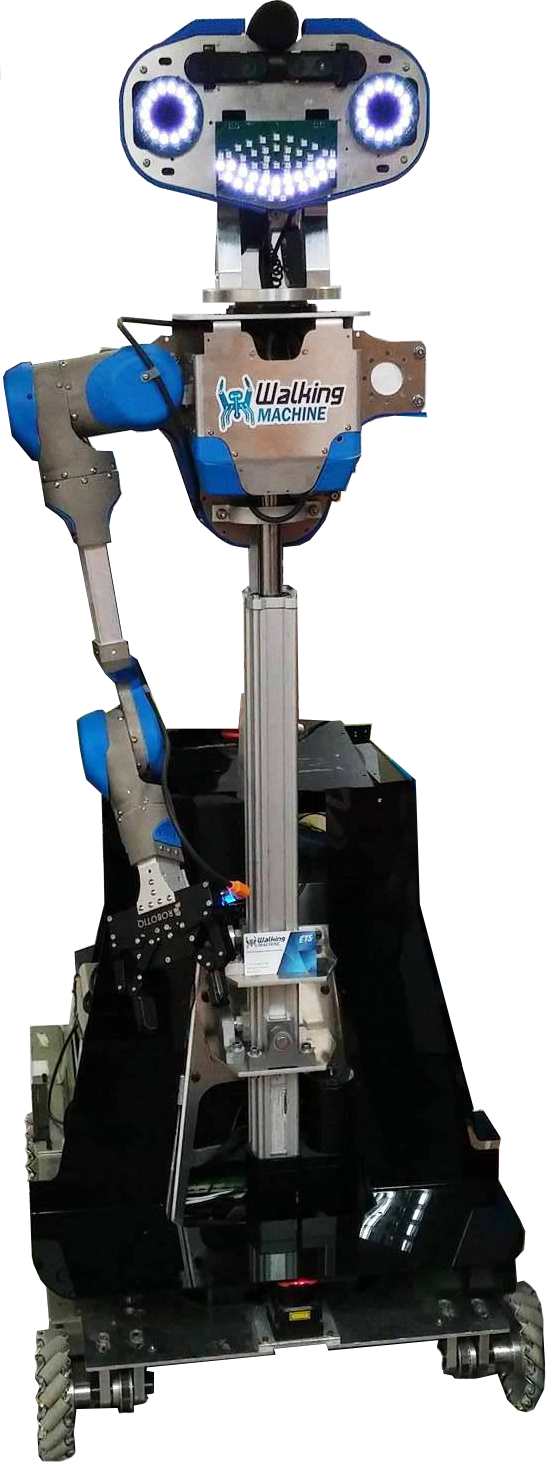
\includegraphics[width=0.20\textwidth]{images/sara_full.png}
	\caption{Robot SARA}
\end{wrapfigure}
\section*{Robot's Software Description}

For our robot we are using the following software:

\begin{itemize}
	\item Platform: Robotic Operating System (ROS) Kinetic on Ubuntu 16.04
	\item Navigation, localization and mapping: RTAB-Map, Gmapping, AMCL, DWA
	\item Face recognition: Cob people detection
	\item Speech recognition: Pocketsphinx
	\item Speech comprehension : LU4R
	\item Speech generation: Svoxpico
	\item Object recognition: Object recognition kitchen
	\item Arms control: Moveit and Kinova API
	\item Task executors: SMACH
\end{itemize}